\documentclass[tikz]{standalone}
\usepackage{tikz}
\usepackage{siunitx}
\DeclareSIUnit\degF{\text{°}F}

\definecolor{codeblue}{RGB}{69, 161, 248}
\definecolor{codegray}{RGB}{40, 40, 40}
\usetikzlibrary{shapes,arrows}
\tikzstyle{decision} = [diamond, draw, fill=codegray, text=white,
    text width=4.5em, text badly centered, node distance=3cm, inner sep=0pt]
\tikzstyle{block} = [rectangle, draw, fill=codeblue,  text=white,
    text width=5em, text centered, rounded corners, minimum height=4em]
\tikzstyle{line} = [draw, -latex']


\begin{document}
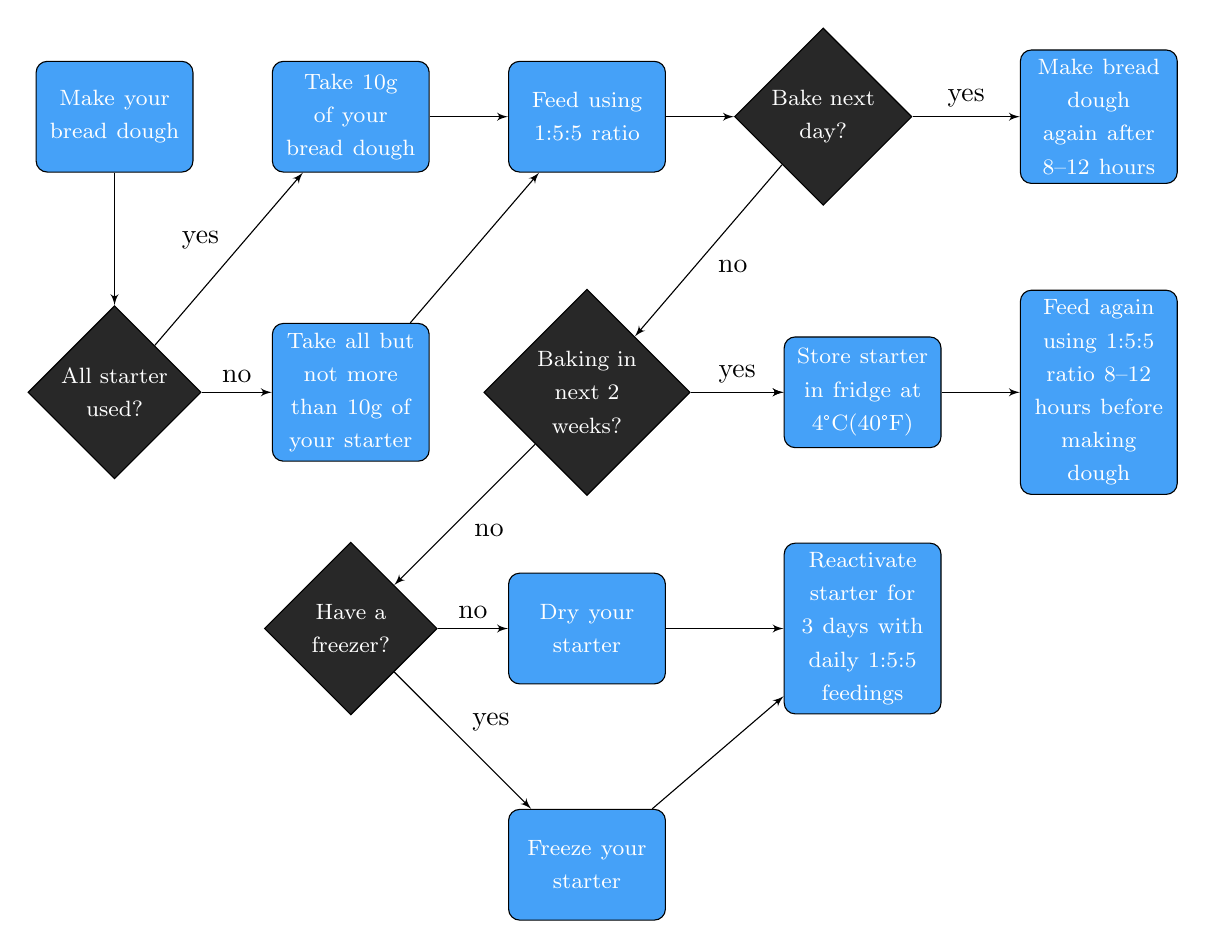
\begin{tikzpicture}[node distance = 3cm, auto]
  \node [block] (init) {\footnotesize Make your bread dough};
  \node [decision, below of=init, node distance=3.5cm] (all_starter_used) {\footnotesize All starter used?};
  \path [line] (init) -- (all_starter_used);
  \node [block, right of=init, node distance=3cm] (use_dough) {\footnotesize Take 10g of your bread dough};
  \node [block, right of=all_starter_used, node distance=3cm] (use_starter) {\footnotesize Take all but not more than 10g of your starter};
  \path [line] (all_starter_used) -- node{yes} (use_dough);
  \path [line] (all_starter_used) -- node{no} (use_starter);
  \node [block, right of=use_dough, node distance=3cm] (feed_starter) {\footnotesize Feed using 1:5:5 ratio};
  \path [line] (use_dough) -- (feed_starter);
  \path [line] (use_starter) -- (feed_starter);
  \node [decision, right of=feed_starter, node distance=3cm] (bake_next_day_check) {\footnotesize Bake next day?};
  \path [line] (feed_starter) -- (bake_next_day_check);
  \node [block, right of=bake_next_day_check, node distance=3.5cm] (make_bread_dough) {\footnotesize Make bread dough again after 8--12 hours};
  \path [line] (bake_next_day_check) -- node{yes} (make_bread_dough);
  \node [decision, right of=use_starter, node distance=3cm] (bake_next_week_check) {\footnotesize Baking in next 2 weeks?};
  \node [block, right of=bake_next_week_check, node distance=3.5cm] (store_fridge) {\footnotesize Store starter in fridge at 4°C(40°F)};
  \path [line] (bake_next_week_check) -- node{yes} (store_fridge);
  \node [block, right of=store_fridge, node distance=3cm] (feed_after_fridge) {\footnotesize Feed again using 1:5:5 ratio 8--12 hours before making dough};
  \path [line] (store_fridge) -- (feed_after_fridge);
  \path [line] (bake_next_day_check) -- node{no} (bake_next_week_check);
  \node [decision, below of=use_starter, node distance=3cm] (freezer_check) {\footnotesize Have a freezer?};
  \path [line] (bake_next_week_check) -- (store_fridge);
  \path [line] (bake_next_week_check) -- node{no} (freezer_check);
  \node [block, right of=freezer_check, node distance=3cm] (dry_starter) {\footnotesize Dry your starter};
  \node [block, below of=dry_starter, node distance=3cm] (freeze_starter) {\footnotesize Freeze your starter};
  \path [line] (freezer_check) -- node{no} (dry_starter);
  \path [line] (freezer_check) -- node{yes} (freeze_starter);
  \node [block, right of=dry_starter, node distance=3.5cm] (reactivate_freezer) {\footnotesize Reactivate starter for 3 days with daily 1:5:5 feedings};
  \path [line] (dry_starter) -- (reactivate_freezer);
  \path [line] (freeze_starter) -- (reactivate_freezer);
\end{tikzpicture}
\end{document}
